\chapter{Materiais e Método}


%---------------------------------------------------------------------------SUB MATERIAIS
\subsection{\textbf{Materiais}}

\par
Em relação ao ambiente de execução, foram utilizados dois ambientes: o primeiro foi o Google Colab para a análise dos resultados e exploração dos dados históricos das ações, utilizando Python em sua versão 3.7.10 (x64); o segundo foi o PyCharm utilizando Python 3.7.0 (x64), destinado para o processamento dos modelos e geração dos resultados. Para possibilitar a implementação das técnicas de Deep Learning (CNN e LSTM) e do modelo Autorregressivo utilizados, bem como a aplicação dos algoritmos e transformações dos dados, algumas bibliotecas da linguagem Python compuseram uma referência base para sua concretização, e estão contidas na tabela abaixo:


%---------------TABLE
\begin{table}[htp]
    \footnotesize
        \caption{Bibliotecas utilizadas, suas respectivas versões e propósitos.}
        \begin{tabular}{cccll}
            \cline{1-3}
            \textbf{Bibliotecas} & \textbf{Versão} & \textbf{Descrição} &  &  \\ \cline{1-3}
            {\fontfamily{cmtt}\selectfont numpy} & 1.19.5 & funções   matemáticas e transformações de matrizes &  &  \\
            {\fontfamily{cmtt}\selectfont matplotlib} & 3.2.2 & plotagem   de gráficos &  &  \\
            {\fontfamily{cmtt}\selectfont pandas\_datareader} & 0.9.0 & carregamento   dos dados históricos, API do yahoo &  &  \\
            {\fontfamily{cmtt}\selectfont pandas} & 1.1.5 & carregamento   e transformações de dados &  &  \\
            {\fontfamily{cmtt}\selectfont sklearn} & 0.22.2.post1 & métricas   para avaliação e pré-processamento dos dados &  &  \\
            {\fontfamily{cmtt}\selectfont datetime} & \textit{defaut} & transformações   de datas &  &  \\
            {\fontfamily{cmtt}\selectfont statsmodels} & 0.10.2 & modelo   Autorregressivo &  &  \\
            {\fontfamily{cmtt}\selectfont keras} & 2.4.3 & modelos CNN e LSTM &  &  \\ \cline{1-3}
        \end{tabular}
        \label{tab:tabela1}
    \center{Fonte: Autor do relatório.}
\end{table}


\par{
Com relação ao hardware referente ao processamento e execução dos algoritmos, o ambiente utilizado foi:}


%---------------TABLE
\begin{table}[htp]
\footnotesize
\centering
\caption{Características de hardware do ambiente de processamento utilizado.}
\begin{tabular}{llcll}
\cline{1-2}
\multicolumn{1}{c|}{CPU} & Intel(R) Core(TM) i7-7700HQ CPU @ 2.80GHz & \textbf{} &  &  \\
\multicolumn{1}{c|}{Memória RAM} & 16GB &  &  &  \\
\multicolumn{1}{c|}{GPU} & NVIDIA GeForce GTX 1050 Ti &  &  &  \\
\multicolumn{1}{c|}{Sistema Operacional (SO)} & Microsoft Windows 10 Pro (x64) &  &  &  \\
\multicolumn{1}{c|}{Versão do SO} & 10.0.19042 N/A compilação 19042 &  &  &  \\
\multicolumn{1}{c|}{Modelo do sistema} & Nitro AN515-51 &  &  &  \\
\multicolumn{1}{c|}{Tipo de sistema} & x64-based PC &  &  &  \\ \cline{1-2}
\end{tabular}
\center{Fonte: Autor do relatório.}
\end{table}


%---------------------------------------------------------------------------SUB MÉTODO
\subsection{\textbf{Método}}

\par
O método empregado visa a mensuração e a comparação entre modelos relacionadas à Séries Temporais Financeiras, tratando-se de um método quantitativo, considerando que utiliza de uma abordagem estatística no que tange à comparação das técnicas existentes, a fim de estabelecer hipóteses de situações potenciais de uso destas, bem como identificá-las mediante análise \cite{wainer}.

\par
As redes neurais testadas (CNN e LSTM) foram treinadas com os preços de fechamento de cada dia dos períodos escolhidos, e então foi testada para um ano posterior ao ano final de treino. As saídas foram numéricas, e então comparadas com os fechamentos reais do ano em questão que foi realizado o teste. Para as saídas geradas, também, foi submetido um algoritmo que compara o preço atual previsto com o preço previsto do dia seguinte, e então classifica-o em “subida” ou “descida”; tais classificações foram comparadas aos movimentos reais obtidos nos fechamentos reais de cada dia, no caso se o preço do dia seguinte foi maior que o atual (subida), ou então foi menor que o atual (descida).

\par
As técnicas de redes neurais CNN e LSTM foram testadas em diferentes períodos, e o experimento foi repetido 10 vezes para cada período devido aos processos estocásticos que ocorrem internamente no funcionamento das redes neurais. Os resultados obtidos foram comparados entre as técnicas, bem como os resultados dos processos de simulação de operação na bolsa de valores.


%---------------------------------------------------------------------------subsub Características dos Dados
\subsubsection{Características dos Dados}


%---------------FIGURE
\begin{figure}[hbt]
\centering
\caption{Dados históricos da ação PETR4.SA (Petrobrás), no ano de 2020.}
  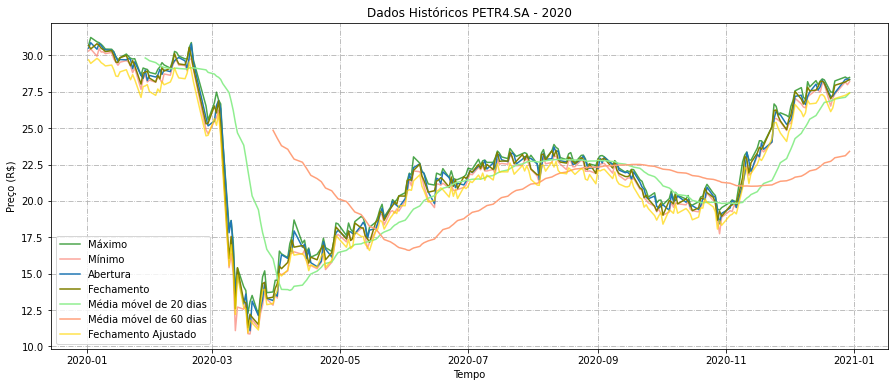
\includegraphics[scale=0.52]{figures/img2.png}
  Fonte: \href{https://finance.yahoo.com/}{Yahoo Finance}. Acesso em 14 mai. 2021.
\end{figure}


%---------------FIGURE
\begin{figure}[H]
\centering
\caption{(a) Altas e baixas; (b) Aberturas e fechamentos; ações PETR4.SA, ano de 2020.}
  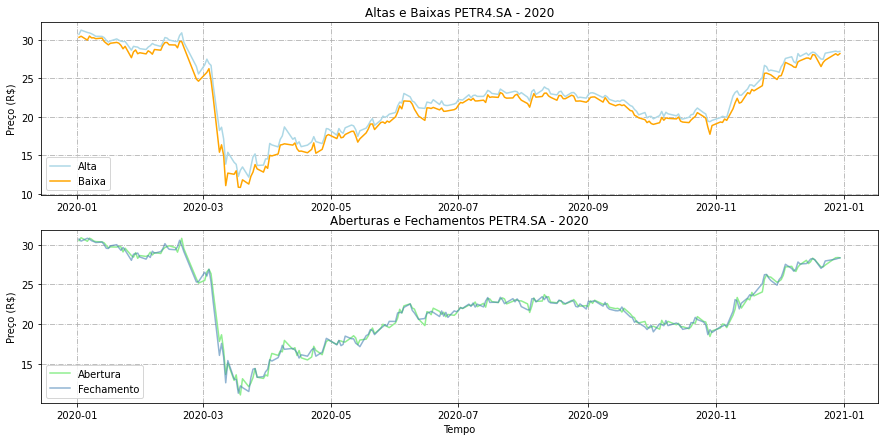
\includegraphics[scale=0.52]{figures/img3.png}
  Fonte: \href{https://finance.yahoo.com/}{Yahoo Finance}. Acesso em 14 mai. 2021.
\end{figure}


%---------------FIGURE
\begin{figure}[H]
\centering
\caption{Dados históricos das cotações em formato de \textit{candlestick}; ações PETR4.SA, ano de 2020.}
  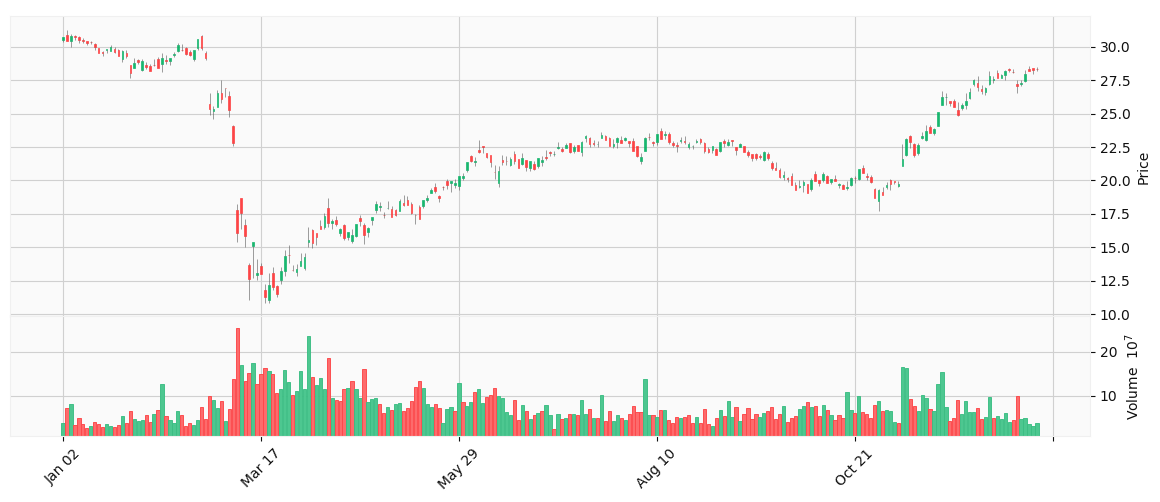
\includegraphics[scale=0.55]{figures/img4.png}
  Fonte: \href{https://finance.yahoo.com/}{Yahoo Finance}. Acesso em 14 mai. 2021.
\end{figure}


%---------------FIGURE
\begin{figure}[H]
\centering
\caption{Retornos diários; ações PETR4.SA, 2020.}
  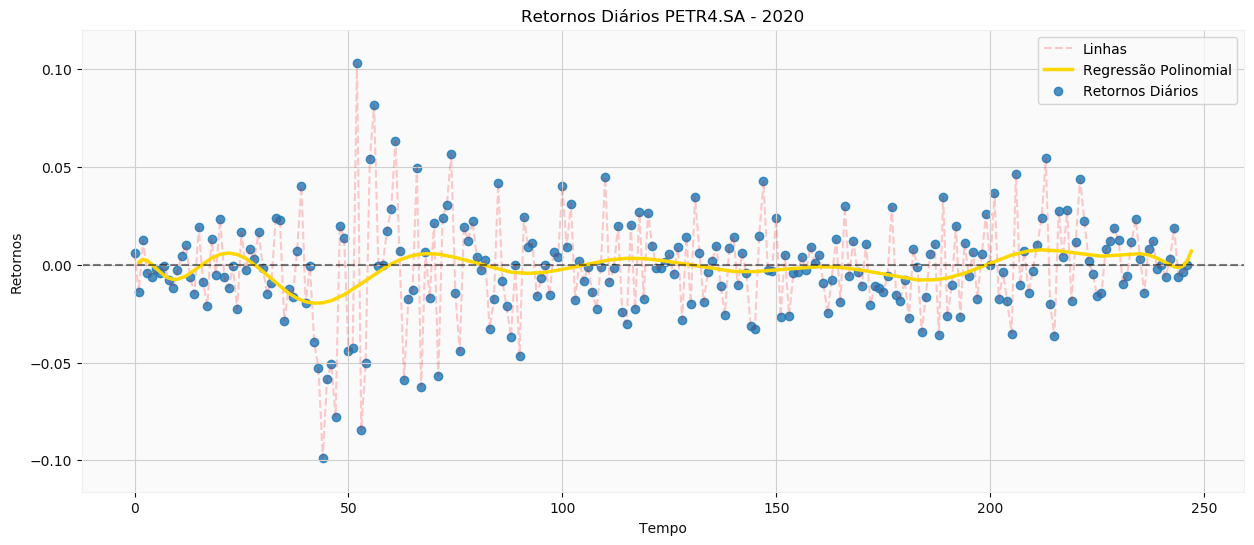
\includegraphics[scale=0.52]{figures/img5.png}
  Fonte: O autor do relatório.
\end{figure}


%---------------TABLE
\begin{table}[H]
\footnotesize
\centering
\caption{Estatísticas sobre os dados históricos da ação PETR4.SA, para o ano de 2020.}
\begin{tabular}{lccll}
\cline{1-3}
\multicolumn{1}{c}{\textbf{Métricas}} & \textbf{2019} & \textbf{2020} &  &  \\ \cline{1-3}
\textit{Contagem} & 247 & 247 &  &  \\
\textit{Média} & 27.248988 & 22.287895 &  &  \\
\textit{Std} & 1.655566 & 4.605092 &  &  \\
\textit{Min} & 23.910000 & 11.290000 &  &  \\
\textit{25\%} & 26.065000 & 19.639999 &  &  \\
\textit{50\%} & 27.129999 & 22.120001 &  &  \\
\textit{75\%} & 28.220000 & 25.710000 &  &  \\
\textit{Max} & \multicolumn{1}{l}{30.969999} & \multicolumn{1}{l}{30.809999} &  &  \\ \cline{1-3}
\end{tabular}
\center{Fonte: Autor do relatório.}
\end{table}


%---------------------------------------------------------------------------subsub Treino e teste do CNN e LSTM
\subsubsection{Treino e teste do CNN e LSTM}

\par
O treino dos modelos, individualmente, foi dividido em diferentes períodos para uma maior variabilidade nos resultados, objetivando submeter o modelo a diferentes situações e registrar seu desempenho. Cada período corresponde a um experimento realizado, seguido da operação simulada na bolsa e a coleta das métricas. Os períodos considerados para treino, teste e simulação de operação de trading, para o CNN e o LSTM foram:


%---------------TABLE
\begin{table}[htp]
\footnotesize
\centering
\caption{Períodos de treino e teste.}
\begin{tabular}{lllll}
\cline{1-4}
\multicolumn{1}{c}{\textbf{Período}} & \multicolumn{1}{c}{\textbf{Treino}} & \multicolumn{1}{c}{\textbf{Teste}} & \multicolumn{1}{c}{\textbf{Resumo}} &  \\ \cline{1-4}
\multicolumn{1}{c}{Período   1} & \multicolumn{1}{c}{01/01/2010    à  31/12/2018} & \multicolumn{1}{c}{01/01/2019    à  31/12/2019} & \multicolumn{1}{c}{2010-2018:   \textit{Treino};  2019: \textit{Teste}} &  \\
\multicolumn{1}{c}{Período   2} & \multicolumn{1}{c}{01/01/2010    à  31/12/2019} & \multicolumn{1}{c}{01/01/2020    à  31/12/2020} & \multicolumn{1}{c}{2010-2019:   \textit{Treino};  2020: \textit{Teste}} &  \\
\multicolumn{1}{c}{Período   3} & \multicolumn{1}{c}{01/01/2010    à  31/12/2018} & \multicolumn{1}{c}{01/01/2020    à  31/12/2020} & \multicolumn{1}{c}{2010-2018: \textit{Treino};  2020:   \textit{Teste}} &  \\ \cline{1-4}
\end{tabular}
\center{Fonte: Autor do relatório.}
\end{table}


%---------------TABLE
\begin{table}[htp]
\footnotesize
\centering
\caption{Períodos de simulação de operação (\textit{trading}).}
\begin{tabular}{lllll}
\cline{1-3}
\multicolumn{1}{c}{\textbf{Período}} & \multicolumn{1}{c}{\textbf{Início   trading}} & \multicolumn{1}{c}{\textbf{Fim   trading}} &  &  \\ \cline{1-3}
\multicolumn{1}{c}{Período   1} & \multicolumn{1}{c}{01/01/2019} & \multicolumn{1}{c}{31/12/2019} &  &  \\
\multicolumn{1}{c}{Período   2} & \multicolumn{1}{c}{01/01/2020} & \multicolumn{1}{c}{31/12/2020} &  &  \\
\multicolumn{1}{c}{Período   3} & \multicolumn{1}{c}{01/01/2020} & \multicolumn{1}{c}{31/12/2020} &  &  \\ \cline{1-3}
\end{tabular}
\center{Fonte: Autor do relatório.}
\end{table}


%---------------TABLE
\begin{table}[H]
\footnotesize
\centering
\caption{Divisão percentual, dos períodos de treino, teste e operação, em percentuais (os intervalos de teste e trading são os mesmos para cada período).}
\begin{tabular}{lllll}
\cline{1-4}
\multicolumn{1}{c}{\textbf{Período}} & \multicolumn{1}{c}{\textbf{Treino}} & \multicolumn{1}{c}{\textbf{Teste}} & \multicolumn{1}{c}{\textbf{Trading}} &  \\ \cline{1-4}
\multicolumn{1}{c}{Período   1} & \multicolumn{1}{c}{89\%} & \multicolumn{1}{c}{11\%} & \multicolumn{1}{c}{11\%} &  \\
\multicolumn{1}{c}{Período   2} & \multicolumn{1}{c}{90\%} & \multicolumn{1}{c}{10\%} & \multicolumn{1}{c}{10\%} &  \\
\multicolumn{1}{c}{Período   3} & \multicolumn{1}{c}{89\%} & \multicolumn{1}{c}{11\%} & \multicolumn{1}{c}{11\%} &  \\ \cline{1-4}
\end{tabular}
\center{Fonte: Autor do relatório.}
\end{table}


%---------------------------------------------------------------------------subsub
\subsubsection{Parâmetros dos modelos utilizados}

\begin{itemize}
\item{CNN}
\end{itemize}
 
\par
A rede foi treinada com o atributo “\textit{close}” de cada dia durante o período de treino, que corresponde ao preço de fechamento da ação naquele dia. As saídas geradas foram números que buscaram prever a ação do dia seguinte. Um algoritmo recebeu tais valores numéricos previstos e retornou as classificações de “alta” ou “baixa” para o dia de hoje, comparando com o preço de amanhã. Abaixo, segue o trecho do código com os parâmetros utilizados nos testes com o CNN:


%---------------CODE
\begin{figure}[hbt]
\caption{Parâmetros utilizados para o treino da rede CNN.}
\lstinputlisting[language=Python]{codes/params1.py}
\center{Fonte: Autor do relatório.}
\end{figure}

\begin{itemize}
\item{LSTM}
\end{itemize}

\par
De maneira semelhante à rede CNN, a rede LSTM foi utilizada para o treino com os preços de fechamentos das ações. A figura abaixo é um trecho de código com a declaração do modelo e os parâmetros utilizados nos testes:


%---------------CODE
\begin{figure}[H]
\caption{Parâmetros utilizados nos testes com a rede LSTM.}
\lstinputlisting[language=Python]{codes/params2.py}
\center{Fonte: Autor do relatório.}
\end{figure}


\begin{itemize}
\item{Modelo \textit{Naive}}
\end{itemize}

\par
O Modelo \textit{Naive} (Modelo “Ingênuo”, do inglês “\textit{naive}”) se refere a um modelo utilizado como base de comparação para as redes neurais. A palavra “ingênuo” se refere à simplicidade do modelo: todas as “previsões” de um período \textit{p} são obtidas por meio do valor do período $p-1$. Dessa forma, todas as previsões são “projeções” dos dados para o futuro; em linhas gerais, representa a confiança de que os dados obtidos no passado se repetirão no presente (daí o termo “ingênuo”).

\begin{itemize}
\item{Modelo Autorregressivo (AR)}
\end{itemize}

\par
Outro modelo utilizado para comparar com os resultados obtidos pelas redes neurais é o modelo Autorregressivo. Este modelo pertence à família de modelos estatísticos tradicionais para a previsão em séries temporais; por ser robusto, foi utilizado neste trabalho para trazer uma base comparativa.

\par
Para o modelo Autorregressivo, foram utilizados 60 dias anteriores ao período de teste e operação para o treino. Por exemplo, para o teste e treino no ano de 2019, o modelo utilizou 60 dias do final de 2018 para treiná-lo. O parâmetro \textit{endog} do modelo foi o conjunto de preços de fechamento, e o \textit{maxlag} foi 60.

%---------------------------------------------------------------------------SUB
\subsection{\textbf{Algoritmos de Trading}}

São os algoritmos que realizam a simulação da operação de trading na bolsa de valores, cada um com uma regra específica associada à tomada de decisão.


%---------------------------------------------------------------------------subsub
\subsubsection{Algoritmo \textit{Classifications Trading} (CT)}

\par
Algoritmo de Trading que utiliza as classificações de “alta” ou “baixa” para o dia seguinte (em relação ao preço de fechamento) para tomar decisões a respeito da compra ou venda de ações \cite{ritzmann}. Resumidamente, o algoritmo irá se basear na previsão do dia de hoje, comparando se o movimento previsto de hoje em relação a amanhã será de baixa ou alta. Por exemplo, o modelo CNN previu o valor R\$ 26,88 para o fechamento de amanhã, e o fechamento de hoje é de R\$ 24,90, logo será classificado como “alta” para hoje, pois amanhã o preço de fechamento subirá, logo o algoritmo fará uma compra.


%---------------FIGURE
\begin{figure}[hbt]
\centering
\caption{\label{figure:figura1}: Fluxograma do algoritmo “\text{\textit{Classifications Trading}}”.}
  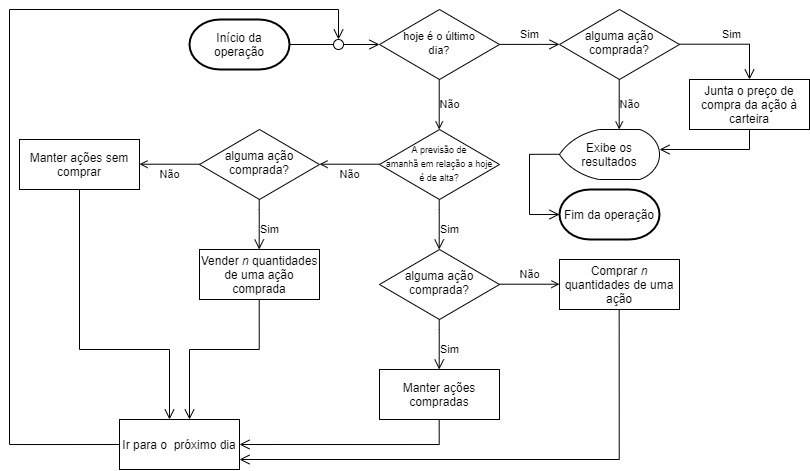
\includegraphics[scale=0.55]{figures/Classifications_Trading.png}
  Fonte: O autor do relatório.
\end{figure}


%---------------PSEUDOCODE
\begin{algorithm}[H]
\caption{Pseudocódigo do algoritmo \textit{classifications\_trading}(\textit{c}, $ \vec{p_c} $, $ \vec{p_p} $)}
\scriptsize
\textbf{Entrada}: Carteira inicial \textit{c}; preços reais de fechamento $ \vec{p_c} $; preços previstos de fechamento $ \vec{p_p} $
\begin{algorithmic}[1]
\footnotesize
\Function{ClassificationsTrading}{\textit{c}, $ \vec{p_c} $, $ \vec{p_p} $}
    \State $ultima\_compra\gets 0$
    \State $acao\_comprada\gets falso$
        \For{$dia$}{$hoje$}{$ultimo\_dia$}
            \If {$hoje == ultimo\_dia$}
                \State $c \gets c + ultima\_compra$
            \Else
                \If {$\vec{p_p}[dia] == subida $}
                    \If {$acao\_comprada == verdadeiro $}
                        \State $continuar$
                    \Else
                        \State $comprar\_acao(n\_acoes)$
                        \State $acao\_comprada = verdadeiro$
                    \EndIf
                \Else
                    \If {$acao\_comprada == verdadeiro $}
                        \State $vender\_acao(n\_acoes)$
                        \State $acao\_comprada = falso$
                    \Else
                        \State $continuar$
                    \EndIf
                \EndIf
            \EndIf
        \EndFor
\EndFunction
\end{algorithmic}
\end{algorithm}


%---------------------------------------------------------------------------subsub
\subsubsection{Algoritmo \textit{Naive Trading} (NT)}


\par
Algoritmo de Trading que utiliza uma técnica ingênua para tomada de decisão. Se o preço de fechamento de ontem for menor que o preço de fechamento de antes de ontem, infere-se que o mercado está em queda, portanto as ações serão vendidas. Caso contrário, ou seja, o preço de ontem é maior que o de antes de ontem, então compramos ações. A ideia desse algoritmo é ter uma base de comparação próxima do real, para os casos de compra e venda sem técnicas sofisticadas e afins, de maneira a averiguar o desempenho de tal técnica em relação às previsões provenientes das redes neurais.


%---------------PSEUDOCODE
\begin{algorithm}[H]
\caption{Pseudocódigo do algoritmo \textit{naive\_trading}(\textit{c}, $ \vec{p_c} $)}
\scriptsize
\textbf{Entrada}: Carteira inicial \textit{c}; preços reais de fechamento $ \vec{p_c} $;
\begin{algorithmic}[1]
\footnotesize
\Function{NaiveTrading}{\textit{c}, $ \vec{p_c} $}
    \State $ultima\_compra\gets 0$
    \State $acao\_comprada\gets falso$
        \For{$dia$}{$hoje$}{$ultimo\_dia$}
            \If {$hoje == ultimo\_dia$}
                \State $c \gets c + ultima\_compra$
            \Else
                \If {$\vec{p_c}[dia-1] > \vec{p_c}[dia-2]$}
                    \If {$acao\_comprada == verdadeiro $}
                        \State $continuar$
                    \Else
                        \State $comprar\_acao(n\_acoes)$
                        \State $acao\_comprada = verdadeiro$
                    \EndIf
                \Else
                    \If {$acao\_comprada == verdadeiro $}
                        \State $vender\_acao(n\_acoes)$
                        \State $acao\_comprada = falso$
                    \Else
                        \State $continuar$
                    \EndIf
                \EndIf
            \EndIf
        \EndFor
\EndFunction
\end{algorithmic}
\end{algorithm}


%---------------------------------------------------------------------------subsub
\subsubsection{Algoritmo \textit{Real Movements Trading} (RMT)}


\par
O algoritmo “\textit{Real Movements Trading}” é, na realidade, o mesmo algoritmo de “Classifications Trading”, com a única diferença que este utiliza os movimentos reais do período de operação, portanto é um algoritmo com 100\% de precisão em relação às operações com lucro. A ideia desse algoritmo é ter uma base de comparação utópica, para um caso perfeito onde saberíamos todos os movimentos reais da bolsa de valores antes mesmo de acontecerem. Por exemplo, o preço de fechamento de amanhã será maior que o de hoje, então o movimento é classificado como “alta”, então o algoritmo efetua a compra de ações para aproveitar o aumento de preço em detrimento de uma compra com valor inferior ao de amanhã; o algoritmo só fará a venda das ações quando o movimento for de “descida”, então venderá todas as ações antes de obter prejuízo.


%---------------------------------------------------------------------------SUB
\subsection{\textbf{Métricas de avaliação utilizadas}}


\par
Os testes com os modelos e as operações foram submetidos à métricas específicas para cada caso. Ao final, foram extraídas as médias e desvio-padrões dos resultados de cada métrica. 


%---------------------------------------------------------------------------subsub
\subsubsection{Métricas de Teste}


\par
As métricas utilizadas para avaliar o desempenho dos modelos em teste, logo após serem treinados e testados durante um ano. As saídas numéricas se referem ao preço de fechamento “previsto” pelo modelo. As saídas categóricas se referem as classificações geradas ao compararem os preços “previstos” para rotulá-las em “alta” ou “baixa”.


%---------------------------------------------------------------------------subsubsub
\subsubsubsection{\textit{Métricas para as Saídas numéricas}}


\begin{itemize}
\item{Coeficiente de determinação (\textit{R squared} ou R2)}
\end{itemize}

É uma medida de ajuste de um modelo linear generalizado, cuja equação é:

\begin{equation}
{\displaystyle SQ_{\text{tot}}=\sum _{i=1}^{n}(y_{i}-{\bar {y}})^{2}}
\end{equation}

Onde \textit{n} é o número de observações, $\mathrm{y_i}$ é o valor observado e \textit{y} é a média das observações.


\begin{itemize}
\item{Erro Quadrático Médio (\textit{Mean Squared Error} ou MSE)}
\end{itemize}

É a média da diferença entre o valor real e previsto, cujo método é:

\begin{equation}
    {\displaystyle EQM({\hat {\theta }})={\frac {1}{N}}\sum _{i=1}^{N}({\hat {\theta _{i}}}-\theta _{i})^{2}}
\end{equation}

Onde $\mathrm{\theta}$ é o valor estimado, $\mathrm{\theta_{i}}$ o valor previsto e \textit{N} o número de observações.


%---------------------------------------------------------------------------subsubsub
\subsubsubsection{\textit{Métricas para as saídas categóricas}}


\begin{itemize}
\item{Medida F (\textit{F1-Score}) \par Medida que utiliza \textit{accuracy}, \textit{precision} e \textit{recall} para gerar um score, cujo método é:}
\end{itemize}


\begin{equation}
F1 = 2 \times \frac{precision \times recall}{precison + recall}
\end{equation}

\begin{itemize}
\item{Acurácia (\textit{Accuracy}) \par Porcentagem de previsões corretas em relação ao total de previsões, cujo método é:}
\end{itemize}


\begin{equation}
accuracy = \frac{TP + TN}{TP + TN + FP + FN}
\end{equation}

\begin{itemize}
\item{Precisão (\textit{Precision}) \par Porcentagem de dados positivos entre todos os classificados como positivos, cujo método é:}
\end{itemize}


\begin{equation}
precision = \frac{TP}{TP+FP}
\end{equation}

\begin{itemize}
\item{Revocação (\textit{Recall}) \par Indica o quão bem o modelo prevê positivos em relação ao total de positivos, cujo método é:}
\end{itemize}


\begin{equation}
recall = \frac{TP}{TP + FN}
\end{equation}


%---------------------------------------------------------------------------subsub
\subsubsection{Métricas para o período de \textit{trading}}

\begin{itemize}
\item{\textit{Carteira final} (CF) \par
Valor da carteira, em R\$, no período final após completar a operação de trading.}
\end{itemize}


\begin{itemize}
\item{\textit{Diferença das carteiras} (DC) \par
Diferença, em R\$, entre a carteira inicial (R\$ 100.000,00) e a carteira final da operação.}
\end{itemize}

\begin{itemize}
\item{\textit{Razão entre as carteiras} (RC) \par
Razão entre a carteira final e a carteira inicial.}
\end{itemize}

\begin{itemize}
\item{\textit{Qtd. De Operações com lucro} (QOL) \par
Dentre as operações realizadas (1 operação é o ato de compra e venda), é o número das que tiveram lucro.}
\end{itemize}


\begin{itemize}
\item{\textit{Qtd. De Operações com perda} (QOP) \par
Dentre as operações realizadas, é o número das que tiveram prejuízo.}
\end{itemize}


\begin{itemize}
\item{\textit{Acurácia de operações com lucro} (AOL) \par
Razão entre as operações com lucro e o total de operações realizadas.}
\end{itemize}


\begin{itemize}
\item{\textit{Ganho médio por operações com lucro, em R\$} (GMO) \par
Dentre as operações com lucro, é a média entre o valor lucrado por operação.}
\end{itemize}


%---------------------------------------------------------------------------SUB
\subsection{\textbf{Ordem dos experimentos realizados}}

\par
Os modelos utilizados, juntamente com os algoritmos de trading e os períodos de treino e operação, seguiram a tabela abaixo, que descreve os experimentos realizados:


%---------------TABLE
\begin{table}[htp]
\footnotesize
\centering
\caption{Algoritmo de \textit{trading} escolhido para cada técnica utilizada para realizar previsões, com o respectivo número de ações negociadas em cada operação, e os períodos diferentes para teste e operação.}
\begin{tabular}{ccccc}
\hline
\textbf{Técnica} & \textbf{Algoritmo   Trading} & \textbf{QAC} & \textbf{Período   Trading} & \textbf{Repetições} \\ \hline
CNN & Classificações & 1500 & Período   1, 2 e 3 & 10   vezes p/ cada período \\
LSTM & Classificações & 1500 & Período   1, 2 e 3 & 10   vezes p/ cada período \\
Modelo   Naive & Classificações & 1500 & 2019   e 2020 & 1   vez p/ cada período \\
Autorregressivo & Classificações & 1500 & 2019   e 2020 & 1   vez p/ cada período \\
Modelo   Naive & Classificações & 1500 & 2019   e 2020 & 1   vez p/ cada período \\
Sem   modelo & Naive   Trading & 1500 & 2019   e 2020 & 1   vez p/ cada período \\
Sem   modelo & Movimentos   Reais & 1500 & 2019   e 2020 & 1 vez p/ cada período \\ \hline
\end{tabular}
\center{Fonte: Autor do relatório.}
\end{table}


%---------------FIGURE
\begin{figure}[hbt]
\centering
\caption{\label{figure:figura1}Fluxograma adaptado dos experimentos realizados, com diagrama incluindo treino e teste de diferentes modelos em diferentes períodos, bem como a operação de \textit{trading} com diferentes algoritmos.}
  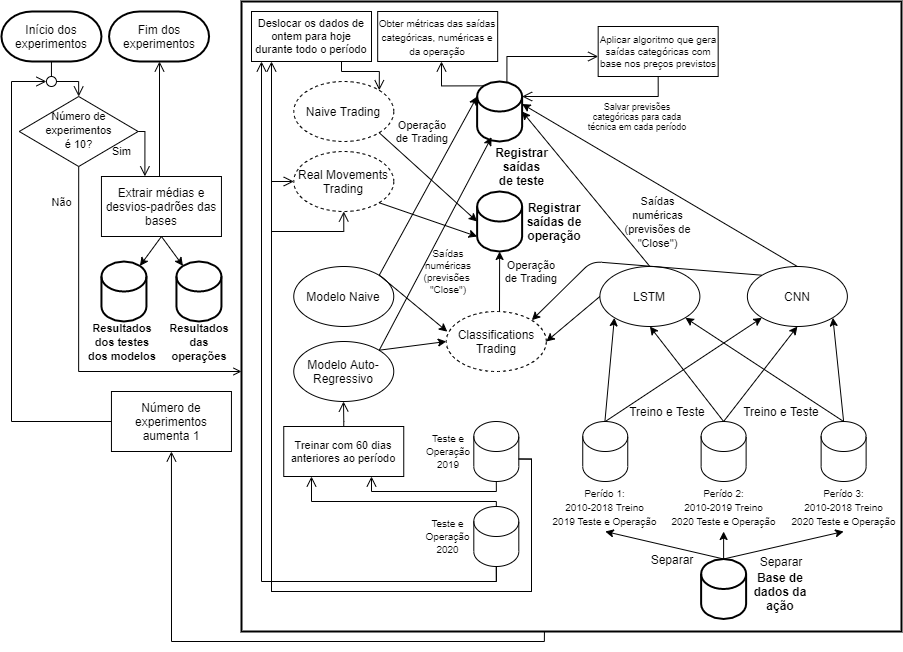
\includegraphics[scale=0.52]{figures/img17.png}
  Fonte: O autor do relatório.
\end{figure}